\documentclass{article}
\usepackage[T1]{fontenc}
\usepackage{lmodern}
\usepackage{graphicx}
\usepackage{amsmath,amssymb}
\usepackage[a4paper,margin=2cm]{geometry}
\usepackage[absolute,overlay]{textpos}
\setlength{\TPHorizModule}{1mm}
\setlength{\TPVertModule}{1mm}
\usepackage[indonesian]{babel}
\usepackage{hyperref}
\setlength{\emergencystretch}{2em}
% unit: Halaman 12

\begin{document}

% === Halaman 12 (llm) ===

“Aman” artinya:

\vspace{95.04mm}

\begin{enumerate}
  \item \textbf{Terjaga kerahasiaannya (confidentiality)}
  \vspace{50mm}
  \item \textbf{Terjaga keasliannya (data integrity)}
  \vspace{50mm}
\end{enumerate}

% deskripsi: Dua kotak teks yang membandingkan teks asli (plainteks) dengan teks terenkripsi (cipherteks) untuk menjelaskan konsep kerahasiaan data.
% bbox normalisasi: [0.0700, 0.2000, 0.5600, 0.4700]
\begin{textblock*}{102.90mm}(14.70mm,59.40mm)
\noindent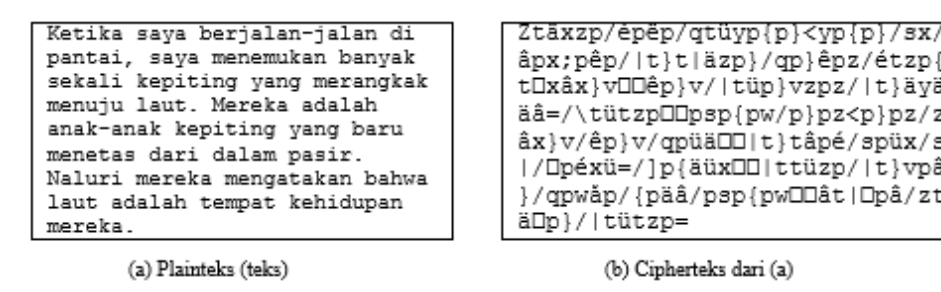
\includegraphics[width=102.90mm,height=80.19mm]{../../images/llm/page_012_img_01.png}%
\end{textblock*}

% deskripsi: Perbandingan dua kotak teks suhu (33 derajat vs 32 derajat) dan dua foto bebek yang hampir identik untuk mengilustrasikan perubahan data (integritas data).
% bbox normalisasi: [0.0900, 0.6300, 0.9600, 0.9500]
\begin{textblock*}{182.70mm}(18.90mm,187.11mm)
\noindent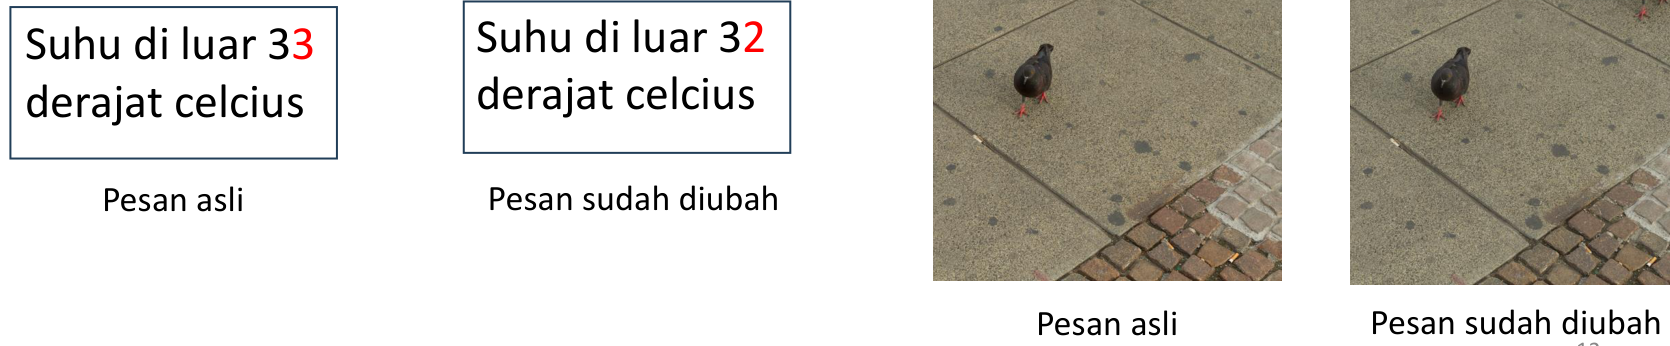
\includegraphics[width=182.70mm,height=95.04mm]{../../images/llm/page_012_img_02.png}%
\end{textblock*}

\end{document}
